\documentclass{wustlthesis}

\setmainfont{Times New Roman}               % Use Times New Roman
\setmathfont{STIXTwoMath}[math-style=ISO]   % Use math font that matches Times New Roman

% Re-calculate the lengths of a text line using the current font
\setlxvchars[\normalfont\normalsize]
\setxlvchars[\normalfont\normalsize]
\checkandfixthelayout[classic]

% Enable refinements of typographics
\usepackage[
    activate=true,
    disable=false,  % enable microtype even in the draft mode
    babel=true,     % enable language-specific kerning.
]{microtype}
\DeclareMicrotypeAlias{Times New Roman}{ptm}

% Hyperlinks
\usepackage{hyperref}
\hypersetup{%
    colorlinks=true,
    linkcolor=black,
    urlcolor=blue,
    citecolor=black,
}
% default URL style
\urlstyle{same}

% Tables
\usepackage{threeparttable}
\usepackage{makecell}  % allow multiple lines in a table cell

% Graphics
\usepackage{graphicx}

% Subcaptions
% The caption format is "Figure 1. Some caption. (A) subcaption. (B) subcaption".
% And the label reference format is "Figure 1A".
\usepackage{subcaption}
\renewcommand\thesubfigure{\Alph{subfigure}}
\renewcommand\thesubtable{\Alph{subtable}}
\captionsetup{subrefformat=parens}

% Allowing subcaptions when all figure panels are combined
% into one source image. Based on https://tex.stackexchange.com/a/255790
\newcommand{\phantomlabel}[1]{%
    \parbox{0pt}{\phantomsubcaption\label{#1}}%
}

% Add a note for figure caption spanning multiple pages
\newcommand{\legendcontdnote}{%
    \sourceatright[2em]{%
        \footnotesize\itshape(legend continued on next page)%
}}
\newcommand{\legendcontdref}[1]{%
    \emph{(\fref{#1} continued)}%
}

% Bibliography
% use BibLaTeX + Biber and Nature citation style.
% some extra configurations:
%   - Hide ISBN and URL
%   - Display DOI
%   - Show up to 9 authors
%   - Enable back references
\usepackage[
    backend=biber,
    style=nature,
    date=year,
    isbn=false, url=false, doi=true,
    minnames=1, maxnames=9,
    backref=true
]{biblatex}
% rename bibliography section name
\DefineBibliographyStrings{english}{
    bibliography = {References},
    backrefpage = {cited on p\adddot},
    backrefpages = {cited on pp\adddot}}
% hide PubMed ID (pmid:xxx) in the bibliography
\DeclareFieldFormat{eprint:pmid}{}

% define the bibliography path
\addbibresource{references.bib}



% Configure title page
\settitle{A Mock Thesis on the Proper Formatting of Dissertations and Theses for\\ Arts \& Sciences Graduate Students}
\setauthor{Paige Turner}
\setthesistype{Dissertation}
\setthesisdegree{Doctor of Philosophy}
\setthesisdegreeabbrv{Ph.D.}
% Degree officially earn date must be in December, May, or August
\setdegreedatemy{May}{2017}
\setthesisadvisorwithtitle{%
    Professor Katherine Davidsen, Chair\\
    Professor Michael Randolf, Co-Chair}
\setthesiscommittee{%
    Katherine Davidsen, Chair\\
    Michael Randolf, Co-Chair\\
    Richard Lewis\\
    Hillary O'Connell\\
    Jack Taylor}
\setthesisschool{Division of Biology and Biomedical Sciences}
\setthesisdepartment{Neurosciences}


% Configure PDF metadata
\hypersetup{
    pdftitle={%
        A Mock Thesis on the Proper Formatting of%
        Dissertations and Theses for Arts \& Sciences Graduate Students%
    },
    pdfauthor={\thesisauthor},
}


% Optional packages that are not required in the real thesis
\usepackage{layout}     % Show page layout
\usepackage{pifont}     % Extra symbols (optional if the main font has the symbols)
\usepackage{emoji}      % Emojis
\usepackage{threeparttable}  % Table
\usepackage{multirow}   % allow multiple lines in a table cell

% Optional styling that is not required in the real thesis
\newcommand*{\file}[1]{\texttt{#1}}


\begin{document}

\thetitlepage                       % Title page
\frontmatter
\thesiscopyright{%                  % Thesis copyright page
    \textcopyright~\degreeearnyear, Paige Turner}

\SingleSpacing*
\setSingleSpace{1.15}
\tableofcontents*                   % Table of contents (ToC)
\listoffigures                      % List of figures (LoF)
\listoftables                       % List of tables (LoT)

\DoubleSpacing
\thesisacknowledgments

An acknowledgments page must be included in your final dissertation or thesis.  If you wish to
include a special dedication you can either use it to close the acknowledgments page or place it on
the page that immediately follows.  The acknowledgments page should be listed in the table of
contents.  Place it after the final list used in the document, and before any dedication, abstract,
or epigraph that is included.

It is appropriate to acknowledge sources of academic and financial support; some fellowships and
grants require acknowledgment.

We offer special thanks to the Washington University School of Engineering for allowing us to use
their dissertation and thesis template as a starting point for the development of this document.

\null\hfill \thesisauthor

\noindent
\textit{Washington University in St.\@ Louis}\\
\textit{May 2017}
    % Acknowledgements
\thesisdedication{%                 % Dedication page
    Dedicated to my parents.}

\begin{abstract}
After removing these comments, begin typing the body of your abstract here, double-spaced.  Your
font should be 12-point (which is the text of this sample paragraph). No part of the abstract
should be bolded. If this is for your master's degree, be sure to change all occurrences of the word
``dissertation'' to display as ``thesis,'' and change ``Doctor of Philosophy'' or ``Doctor of
Liberal Arts'' to ``Master of Arts,'' ``Master of Liberal Arts,'' or ``Master of Fine Arts,''
whichever applies.  In the abstract heading above, make sure you use the year your degree is to be
officially earned. Be sure to use your full name as it is recorded in WebSTAC, your dissertation or
thesis advisor's full name(s) wherever appropriate, and the correct title of your degree whenever
referencing it.  The title of your degree will not always be the same as the title of your
department or program, so please check with your departmental administrative assistant and
advisor(s) to be sure you are using the correct degree title.  Please note that an abstract is
required for all dissertation submissions in ProQuest. An abstract is optional for master's thesis
submissions.
\end{abstract}

\mainmatter
\pagestyle{main}
\chapter{Parts of the Dissertation}
\label{chap:dissertation-parts}

This chapter describes the components of a dissertation.
You may not have to include all components described here, but you must follow the prescribed order for the components you do include.
On \pref{tab:include}, \tref{tab:include} lists the required and optional components in the order that they should appear.
Your manuscript should include three main parts: the front matter, the body, and the back matter.
Each of these parts is described below.

\section{Front Matter}

The front matter includes all material that appears before the beginning of the body of the text.
Number all front matter pages (except the title page and the optional copyright page) with lowercase roman numerals, starting with ii, centered just above the bottom margin.
Each of the following sections should begin on a new page.

\subsection{Title Page}

Format the title page so that it is centered vertically and horizontally on the page with equal amounts of white space from top and bottom margins.
Include a one-inch margin on all sides.
Use a 12-point regular font.
The date on the title page should reflect the month and year the degree is to be officially earned, and should be one of the following months: December, May, or August.
Do \underline{not} include a page number on the title page.
See \hyperref[app:degree-program]{Appendix} for further details.
In most cases your dissertation title should be in ``Title Case'' unless a specific format is required by your discipline.
Be certain to use your own full name (as recorded in \href{https://acadinfo.wustl.edu/}{WebSTAC}).
Following the dissertation chair or co-chair, the faculty should be listed alphabetically by last name.

\begin{table}
	\caption[%
        Required and Optional Thesis Components (NOTE: If you have a multi-lined table label/title,
        then the 2\textsuperscript{nd} and all additional lines should align with the first line, just like this one;
        also, be sure that no words display to the far right hand side where the page numbers for
        your tables display, just as shown in this example.)
    ]{The following items may be included in your dissertation or thesis, in the order in which they are listed.
    Any optional components, if used, \underline{must} be included in the table of contents, unless noted below.}
  \label{tab:include}
  \centering
  \DoubleSpacing

  % Because Times New Roman doesn't have checkmark symbol,
  % Use the checkmark symbol from pifont
  \newcommand{\mycheckmark}{\ding{52}}

  \footnotesize
  \begin{threeparttable}[b]
  \begin{tabular}{@{}ccccc@{}}
  \toprule
    \textbf{Major Part} &
    \makecell[b]{\textbf{Thesis} \\ \textbf{Component}} &
    \textbf{Required} &
    \textbf{Optional} &
    \textbf{Page Numbering} \\
  \midrule

  Front Matter & Title page & \mycheckmark & & counted, not numbered \\
  & Copyright page & & \mycheckmark & neither counted, nor numbered \\
  & Table of Contents & \mycheckmark & & begins on page number \underline{ii} \\
  & List of Figures & & \mycheckmark & [lowercase Roman numerals continue] \\
  & List of Illustrations & & \mycheckmark & [lowercase Roman numerals continue] \\
  & List of Tables & & \mycheckmark & [lowercase Roman numerals continue] \\
  & List of Abbreviations & & \mycheckmark & [lowercase Roman numerals continue] \\
  & Acknowledgments & \mycheckmark & & [lowercase Roman numerals continue] \\
  & Dedication\tnote{*} & & \mycheckmark & [lowercase Roman numerals continue] \\
  & Abstract page & & \mycheckmark & [lowercase Roman numerals continue] \\
  & Preface & & \mycheckmark & [lowercase Roman numerals continue] \\
  Body & Epigraph\tnote{*} & & \mycheckmark & begins on a page numbered \underline{1} \\
  & Chapters & \mycheckmark & & [Arabic numerals begin or continue] \\
  Back Matter & References\tnote{**} & \mycheckmark & & [Arabic numerals continue] \\
  & Appendices & & \mycheckmark & [Arabic numerals continue] \\
  & Curriculum Vitae\tnote{***} & & \mycheckmark & [Arabic numerals continue] \\
  \bottomrule
  \end{tabular}
  \begin{tablenotes}
    \footnotesize
    \item[*] Do not include in the table of contents.
    \item[**] There are two options for the placement of references; they can be listed at the end of each chapter, or at the end of the document.
    \item[***] Do not put your Social Security Number, birthdate, or birthplace on your CV.
  \end{tablenotes}
  \end{threeparttable}
\end{table}

\subsection{Copyright Page}

It is always suggested that upon completion of the text, the student add the copyright symbol © with the year and the student's name on one line, on a page following the title page.
Format your copyright page exactly as it is shown in this template.

\vspace{\onelineskip}
\noindent
\textit{Example:}

\centerline{\textcopyright\ 2022, Paige Turner}
\vspace{\onelineskip}

Once you create a work, it is automatically protected by U.S.\@ copyright law with you as the author.
You do not need to register the copyright with the U.S.\@ Copyright Office, though doing so provides certain advantages.
More information about copyright registration can be found at \href{http://libguides.wustl.edu/copyright/registration}{http://libguides.wustl.edu/copyright/registration}.

\subsection{Table of Contents}

The words ``Table of Contents'' must appear in chapter title style at the top of the page.
It must include the page numbers of all front and back matter elements, unless otherwise specified.
The table of contents must include the page numbers of all chapters and sections of your dissertation.
In addition, it may include the page numbers of all subsections.
Chapter titles may be typed in plain or bold font.
All titles and headings must be followed by a page number.

Make certain that any long titles align nicely with the body of text.
Multi-lined chapter titles or section titles should break at a logical point and align in a manner allowing the titles to be read clearly, without confusion.
Sometimes this will mean forcing a line break at a logical point and relies on your own good judgment.

\subsection{List of Figures}

If one or more figures are used in the document, there must be a list of all figures.
The list should be spaced at 1.15.
Begin each listing on a new line.
Format the list of figures the same way the table of contents is formatted, but put the words ``List of Figures'' in the heading.

\subsection{List of Tables}

If one or more tables are used in the document, there must be a list of all tables.
The list should be spaced at 1.15.
Begin each listing on a new line.
Format the list of tables the same way the table of contents is formatted, but put the words ``List of Tables'' in the heading.

\subsection{List of Abbreviations}

Include a list of abbreviations only if you use abbreviations that are not common in your field.
Arrange the list alphabetically.
Type the words ``List of Abbreviations'' in chapter title style at the top of your list.

\subsection{Acknowledgments}

An acknowledgments section must be included.
Use it to thank those who supported your research through contributions of time, money, or other resources.
Some grants require an acknowledgment.
Type the word ``Acknowledgments'' in chapter title style at the top of your page.
If the acknowledgments fill more than one page, put the heading only on the first page.

\subsection{Dedication}

The dedication page is optional.
If you decide to include a separate dedication page, make it short and center it on the page, both horizontally and vertically.
Do not include it in your table of contents.
See \pref{thesisdedication} for more detailed information.

\subsection{Abstract Page}

An abstract page is optional in the dissertation, but will be required when you submit your manuscript electronically.
Format the abstract page precisely as shown in the front matter of this document.
See \Aref{app:degree-program} for further details.

\subsection{Preface}

A preface is optional.
If you include a preface, use it to explain the motivation behind your work.
Format the preface the same way the acknowledgments section is formatted, but use the word ``Preface'' in the heading.

\section{Body of the Dissertation}

The body of the dissertation should be divided into chapters, sections, and subsections as required by your discipline, and should be numbered as in this template.
Divisions smaller than subsections may be used, but they should not be labeled with numbers (see \Sref{subsec:subsection-headings-numbering} for more information).

\section{Back Matter}

The back matter includes all material that appears after the body of the text.

\subsection{References/Bibliography/Works Cited}

There are two options for the placement of references; they can be listed at the end of each chapter or at the end of the document.
What you call this section and how you format it should follow the usual convention of your discipline and be acceptable to your committee.
Depending on how you title and where you place this section, type the appropriate words in either the section heading or chapter title format at the top of a new page.
Single-space your citations and skip a line between each one.
Regardless of where you choose to place your references, they must be listed in the table of contents.
If placed at the end of your document, this section should follow the conclusion of the text.

\subsection{Appendices}

Appendices may be used for including reference material that is too lengthy or inappropriate for the dissertation body.
If one appendix is included, an appendix title is optional.
If more than one appendix is included, each one should be titled and lettered.
In general, appendices should be formatted like chapters.
However, they may be single-spaced and/or include photocopied or scanned materials.
If these are used, you must add page numbers at the bottom, putting those page numbers in square brackets to indicate that they are not part of the original document.

\subsection{Curriculum Vitae}

Including a Curriculum Vitae (CV) with your dissertation or thesis is optional.
If you choose to include your CV, it should include your name, the month \& year you will be earning your degree, and relevant academic and professional achievements.
It may also include your publications and professional society memberships.
If included, your vita should be the last page(s) of your document.
Note that personally identifiable information such as birth date, place of birth, and social security number should \underline{NOT} be included.

\chapter{Dissertation or Thesis Format}
\label{chap:dissertation-format}

The following guidelines offer you some degree of flexibility in formatting your thesis or dissertation.
Whichever options you choose to use, you must use them consistently throughout the document.

\section{Margins}

Your printed output must reflect physically measurable top, bottom, left, and right margins of 1 inch.
Some systems' settings produce varying results when printing to different printers, so be sure to measure your output.
Remember, nothing, not even page numbers, should print in the margins.

\section{Page Numbers}

All pages numbers should be placed on the center of each page immediately above the bottom margin.
Number all pages in your document except for the title page and the optional copyright page which might follow the title page.
Number the ``front matter'' pages (i.e., the pages that come prior to the main body of text, prior to chapter 1) with lowercase roman numerals, starting with ii (remember, the title page is counted but not numbered, and the copyright page is neither counted nor numbered).
The body of the dissertation or thesis should be numbered with Arabic numerals starting with 1 and should begin on the epigraph page (optional), the introduction, if one is used, or on the first page of the first chapter.
Options are summarized in \tref{tab:include} on page two.

\section{Text}

This template uses a 12-point, Times New Roman font throughout and is recommended for your dissertation or thesis.
However, should you choose to use a different font, you should match the font size as close as possible.
Use double-spacing for body text.
Use either left justification with a ragged right edge or full justification.

\section{Chapter Titles}

Begin each chapter on a new page.
You may start the chapter title below the top margin or you may leave some space and start the chapter title up to 3 inches from the top edge of the page.
The font size for chapter titles should be no larger than 24.
There are two options for formatting the chapter title:

\begin{enumerate}
	\item Type the word ``Chapter'' followed by the chapter number, skip a line, and type the chapter title on the following line; or
	\item Type the chapter number followed by the chapter title, all on the same line.
\end{enumerate}

\section{Section Headings \& Numbering}

Headings may be typed above or on the same line as the sections they label.
Type the chapter number and section number before the section title.
The font size for section headings should be no larger than 18.

\subsection{Subsection Headings \& Numbering}
\label{subsec:subsection-headings-numbering}

This should follow the usual convention of your discipline and be acceptable to your committee; if your discipline calls for them they must be in included in the table of contents.
Type the chapter number, section number and subsection number before the subsection title.
The font size for subsection headings should be no larger than 14.

\subsubsection{Headings for Divisions Smaller than Subsections}

Do not number headings for divisions smaller than subsections.
These are not included in the table of contents.
Headings may be typed above or on the same line as the sections they label.
Divisions smaller than subsections should be the same font size as the body text.

\section{Figures and Tables}

There are two options for numbering your figures and tables; choose one and be consistent in its use throughout your document.
In either case, the name and description of the figure or table should be single spaced and can be a smaller font size.

\begin{enumerate}
	\item Maintain a separate numbering sequence for your list of figures and list of tables.
Label figures with the word ``Figure'' and tables with the word ``Table''; or
	\item Label both figures and tables with the word ``Figure'' and maintain one numbering sequence.
\end{enumerate}

Place figures and tables as close to their reference in the text as possible.
Do not let figures or tables spill out into the margins.

\begin{enumerate}
	\item Place the figure number and title below each figure (or table labeled as a figure).
	\item Place the table number and title above each table labeled as a table.
\end{enumerate}

\begin{figure}
    
\includegraphics{figures/just-a-figure}
    \captionstyle{\raggedright}
    \caption[Left justified figure]{You can left justify your figure.}
    \label{fig:left-justified}
\end{figure}

\begin{figure}
    \centering
    
\includegraphics{figures/just-a-figure}
    \caption[Centered figure]{You can center your figure.}
    \label{fig:centered}
\end{figure}


\section{Lists}

You may include lettered, numbered, or bulleted lists in your document.
Use consistent punctuation and capitalization throughout each list.
Lists may be indented.

\section{Footnotes and Endnotes}

You may use footnotes or endnotes for brief notes that are not appropriate for the body of the text.\footnote{The use of endnotes and footnotes should follow the usual convention of your discipline and be acceptable to your committee.}
Use either footnotes or endnotes consistently throughout your dissertation or thesis.
Endnotes are positioned at the end of each chapter.
Single-space within each footnote or endnote.
Footnotes should be numbered consecutively within a chapter; numbers should restart with each new chapter.
Endnotes should be numbered consecutively through the entire body of your dissertation or thesis.

\section{Quotations}

You must use quotation marks and parenthetical references to indicate words that are not your own.
Put quotation marks around short quotes.
Put long quotes in separate single-spaced paragraphs, indented up to 1 inch from the left margin (these are called block quotations).
Kate Turabian, editor of official publications and dissertation secretary at the University of Chicago for over 25 years, distinguishes short and long quotes as follows:

\begin{quote}
    Short, direct prose quotations should be incorporated into the text of the paper and enclosed in
    double quotation marks: ``One small step for man; one giant leap for mankind.'' But in general a
    prose quotation of two or more sentences which at the same time runs to four or more lines of
    text in a paper should be set off from the text and indented in its
    entirety \ldots\ \cite{Turabian}
\end{quote}

\section{Equations}

Equation numbering and formatting should follow the usual convention of your discipline and be acceptable to your committee.

Equations may be set in-line with the text or numbered and placed in separate paragraphs.
Use the same numbering style for equations as you would for figures and tables.
Here is an example of an equation set in-line with a paragraph: $E = mc^{2}$.
Here is an example equation placed in a separate paragraph:

\begin{align}
	E = mc^{2}
\end{align}

\chapter{{\LaTeX}\ Specific Usage}

This template is heavily built on \href{https://www.ctan.org/pkg/memoir}{\texttt{memoir}} package.
Check out \texttt{memoir}'s documentation for its detailed usage and available customizations.

The thesis style is defined in the document class at \file{wustlthesis.cls}.
Since the school guideline is quite lenient, \texttt{wustlthesis} only contains minimal definition and has minimal required packages.
Packages that implement figures with multiple panels, table styling, hyperlinks, bibliography, and many other commonly used features are \emph{not} included in this document class.
You should feel free to use packages of your choice to enable those features.
Please check their compatibility with memoir through their documentations.

If you want to use the style of this thesis example, \file{thesis.tex} has some opinionated setup of the aforementioned features and you can find some showcases below.


\section{Figures}
Common file formats (PDF, PNG, and JPG) are supported.
Vector figures should be stored as PDF files to prevent pixelation.
For example, \fref{fig:vector} is a vector figure.

\begin{figure}[tb]
  \centering
  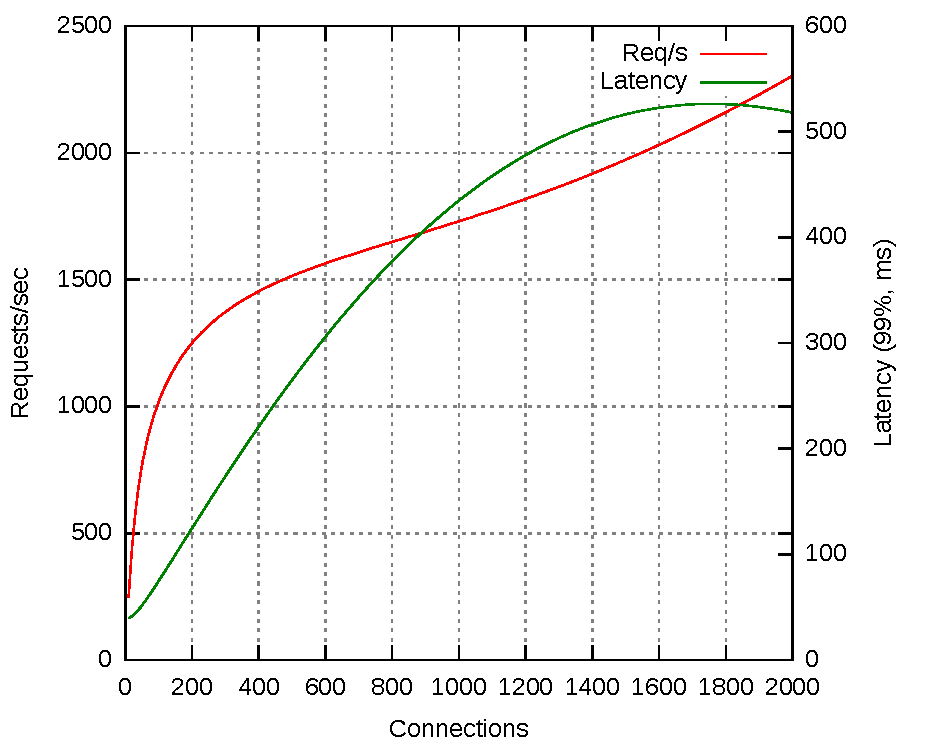
\includegraphics[width=0.6\textwidth]{figures/just-a-plot}
  \caption{Example vector figure in PDF.}
  \label{fig:vector}
\end{figure}



\section{Subfigures and subtables}
If a figure has multiple panels (subfigures), \texttt{subcaption} package is used to enable the correct references for subfigures.
Use \cmd{\fref}\marg{labstr} to refer to the full figure and \cmd{\fref}\marg{sublabstr} to refer to a specfic panel of that figure.
Use \cmd{\subcaptionref}\marg{sublabstr} to refer to just the panel number.
For example, \fref{fig:subfigure-demo} has two panels, \subcaptionref{fig:subfigdemo-cat} and \subcaptionref{fig:subfigdemo-dog}.
\fref{fig:subfigdemo-cat} refers to the cat panel.
This example explicitly creates the panel numbers since figures often have their panel numbers embedded.

\begin{figure}[t]
    \begin{subfigure}[b]{.5\linewidth}
        \centering
        \textbf{\sffamily A}\\[-0.5\onelineskip]
        \HUGE \emoji{cat}\\
        \emoji{cat-face}
        \phantomlabel{fig:subfigdemo-cat}
    \end{subfigure}%
    \begin{subfigure}[b]{.5\linewidth}
        \centering
        \textbf{\sffamily B}\\[-0.5\onelineskip]
        \HUGE \emoji{dog}\\
        \emoji{dog-face}
        \phantomlabel{fig:subfigdemo-dog}
    \end{subfigure}
    \caption[Two animals and their emojis.]{%
        Two animals and their emojis.
        \subref{fig:subfigdemo-cat} cats and \subref{fig:subfigdemo-dog} dogs.
    }
    \label{fig:subfigure-demo}
\end{figure}

Similarly, multiple tables can be grouped together as one using the same method. For example, see \tref{tab:subtable-demo}, which has two panels \subcaptionref{tab:subtab-a} and \subcaptionref{tab:subtab-b}.

\begin{table}[b]
    \centering
    \caption{Another table with two panels: \subref{tab:subtab-a} first and \subref{tab:subtab-b} second panel}
    \label{tab:subtable-demo}

    \begin{subtable}{0.5\linewidth}
        \centering
        \subcaption{First}\label{tab:subtab-a}
        \begin{tabular}{lc} \toprule
        A legendary table & 5 \\
        with two lines    & 6 \\ \bottomrule
        \end{tabular}
    \end{subtable}%
    \begin{subtable}{0.5\linewidth}
        \centering
        \subcaption{Second}\label{tab:subtab-b}
        \begin{tabular}{lc} \toprule
        A legendary table & 5 \\
        with two lines    & 6 \\ \bottomrule
        \end{tabular}
    \end{subtable}
\end{table}


\subsection{Figures with multiple panels merged into one source}
Sometimes the figure has already merges multiple panels and it's hard to split the panels into individual sources.
In this case, the panel numbers can be created using \cmd{\phantomlabel}\marg{labstr}.
For example, both \fref{fig:subfigure-demo} and \ref{fig:cell-cycle-mitosis} create panel numbers using this approach.


\subsection{Long figure legends spanning over the next page}
In some cases, the multi-panel figures may not have the vertical space to fit its legend, so the text overflow to the next page.
The text overflow can be achieved by using \cmd{\legendcontdnote} at the end of the first half of the legend (following the figure) and \cmd{\legendcontdref}\marg{labstr} at the beginning of the second half of the legend (usually at the next page).
\cmd{\legendcontdnote} inserts the ``\emph{(legend continued on next page)}'' mark right aligned at the end of the line or a new line.
\cmd{\legendcontdref} inserts the ``\emph{(Figure X continued)}'' mark.
Their style can modifyied by redefining the commands.

For example, \fref{fig:cell-cycle-mitosis} spans over two pages. Note how the two adjacent figure environments are constructed (and their figure placement specifiers).

\begin{figure}[p]
    \centering
    \phantomlabel{fig:mitosis-prophase}
    \phantomlabel{fig:mitosis-prometaphase}
    \phantomlabel{fig:mitosis-metaphase}
    \phantomlabel{fig:mitosis-anaphase}
    \phantomlabel{fig:mitosis-telophase}
    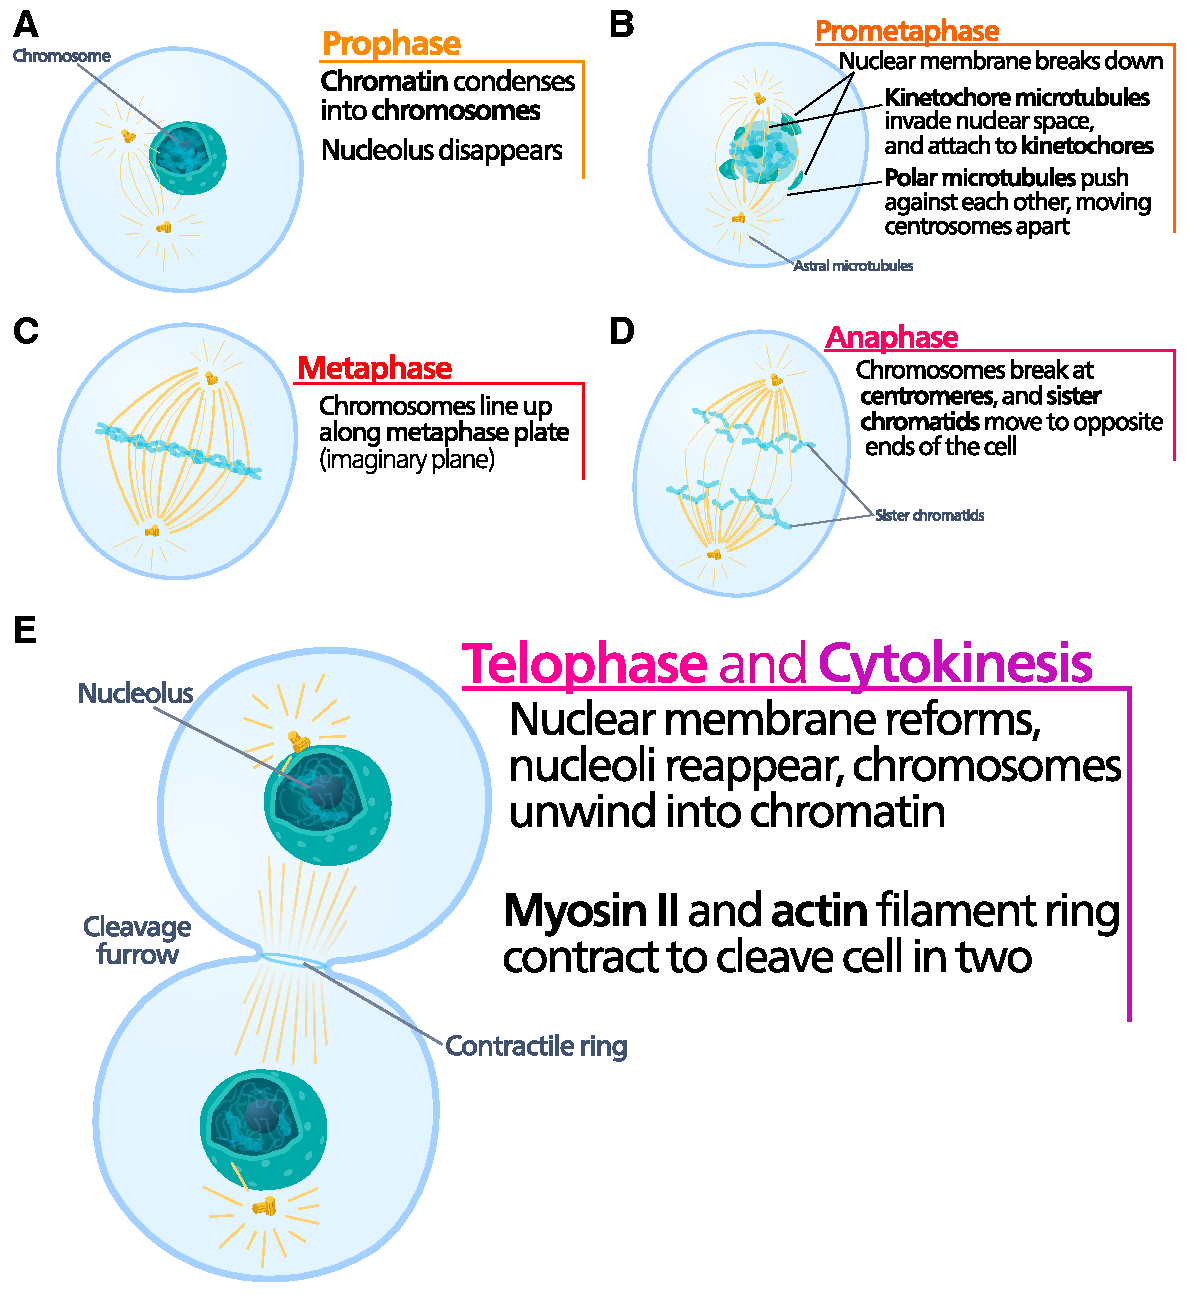
\includegraphics[width=\linewidth]{figures/cell-cycle-mitosis.pdf}
    \caption[Stages of mitotic phase of the cell cycle]{%
        Overview of different stages in the mitotic (M) phase of the animal cell cycle.
        Stages are defined based on the completion of a set of activities.
        \href{https://commons.wikimedia.org/wiki/File:Animal_cell_cycle-en.svg}{Figures} are made by Kelvin Ma (Kelvinsong; Kelvin13), \href{https://creativecommons.org/licenses/by/3.0}{CC BY 3.0}, via Wikimedia Commons.
        Text is copied from the \href{https://en.wikipedia.org/wiki/Mitosis}{Mitosis} page of Wikipedia.
        \subref{fig:mitosis-prophase}
        During prophase, which occurs after G\textsubscript{2} interphase,
        the cell prepares to divide by tightly condensing its chromosomes and initiating mitotic spindle formation.
        \subref{fig:mitosis-prometaphase}
        During prometaphase, the nuclear membrane breaks apart into numerous ``membrane vesicles'', and the chromosomes inside form protein structures called kinetochores.
        \legendcontdnote
    }
    \label{fig:cell-cycle-mitosis}
\end{figure}
\begin{figure}[t]
    \centering
    \legend{%
        \legendcontdref{fig:cell-cycle-mitosis}
        \subref{fig:mitosis-metaphase}
        During metaphase, the two centrosomes begin pulling the chromosomes towards opposite ends of the cell. The resulting tension causes the chromosomes to align along the metaphase plate or equatorial plane.
        \subref{fig:mitosis-anaphase}
        During anaphase, the replicated chromosomes are split and the newly-copied chromosomes are moved to opposite poles of the cell.
        \subref{fig:mitosis-telophase}
        During telophase, the effects of prophase and prometaphase (the nucleolus and nuclear membrane disintegrating) are reversed.
        Telophase is followed by cytokinesis, a separate process necessary for completing cell division.
    }
\end{figure}


\section{Tables}
Both examples (\tref{tab:include} and \ref{tab:nsf-sed}) use the \texttt{threeparttable} environment to format the table and allow table notes.
There are many packages available to manage tabular environments and they are generally compatible to this thesis document class.
For more sophisticated formattings, check out \texttt{memoir}'s documentation.

\begin{table}[tb]
    \centering
    \caption[Definite postgraduation commitments of doctorate recipients]{%
        Definite postgraduation commitments of doctorate recipients,
        by citizenship status and major field of study in 2019.
        Source: National Center for Science and Engineering Statistics, Survey of Earned Doctorates, National Science Foundation
        (\href{https://ncses.nsf.gov/pubs/nsf21308/}{link}; Table 51).
    }
    \label{tab:nsf-sed}
    \begin{threeparttable}[b]
    \begin{tabular}{llrrrrrrr@{}}
    \toprule
    Citizenship & Field & Total &
        Postdoc & Academia & Industry\tnote{a} & Other\tnote{b} & Abroad\\
    \midrule
    \multirow{3}{*}{\begin{tabular}[c]{@{}l@{}}All recipients\tnote{c}\end{tabular}}
        & Bio./biomed. & 5,054 &
            3,426 & 442 & 892 & 294 & 332 \\
        & Health & 1,525 &
            538	& 492 & 220 & 275 & 141\\
        & Comp./info. & 1,414 &
            276 & 254 & 789 & 95 & 161\\
    \midrule
    \multirow{3}{*}{\begin{tabular}[c]{@{}l@{}}U.S. citizen\\or PR\end{tabular}}
        & Bio./biomed. & 3,860 &
            2,536 & 385 & 679 & 260 & 118\\
        & Health & 1,248 &
            375 & 454 & 160 & 259 & 14\\
        & Comp./info. & 557 &
            102 & 133 & 247 & 75 & 23\\
    \midrule
    \multirow{3}{*}{\begin{tabular}[c]{@{}l@{}}Temporary\\visa holder\end{tabular}}
        & Bio./biomed. & 1,180 &
            882 & 55 & 212 & 31 & 213\\
        & Health & 275 &
            163 & 37 & 59 & 16 & 124\\
        & Comp./info. & 851 &
            173 & 120 & 540 & 18 & 136\\
    \bottomrule
    \end{tabular}
    \begin{tablenotes}
    \item[a] Includes doctorate recipients who indicated self-employment.
    \item[b] Includes doctorate recipients who indicated government, nonprofit, elementary or secondary school, or other employment and those with unknown employment.
    \item[c] Includes respondents who did not report citizenship status.
    \end{tablenotes}
    \end{threeparttable}
\end{table}


\section{Bibliography and Citations}
The \texttt{wustlthesis} document class itself does not implement any bibliography settings or styles, so any tool stack can be used together with it.

In this example, the bibliography is managed by \href{http://biblatex-biber.sourceforge.net/}{Biber} and \href{https://www.ctan.org/pkg/biblatex}{BibLaTeX} (not BibTeX), which support Unicode and more formatting options.
If \href{https://www.zotero.org/}{Zotero} is your reference manager, check out \href{https://retorque.re/zotero-better-bibtex/}{Better BibTeX} plugin for Zotero to enable more seamless integration with BibLaTex (and BibTeX).

Regardless of the tool stack in use, the citation commands should be the same, e.g., \cmd{\cite}\marg{key} and \cmd{\citeauthor}\marg{key}.
For example, this paper by \citeauthor{Jinek2012} demonstrated CRISPR can cut DNA at specific nucleotide sequences \cite{Jinek2012}.


\section{Equations}
See Equation~\ref{eq:maxwell}.

\begin{equation}
    \label{eq:maxwell}
    \begin{aligned}
    \frac{\partial\mathcal{D}}{\partial t} & = \nabla\times\mathcal{H},   & \text{(Loi de Faraday)}\\
    \frac{\partial\mathcal{B}}{\partial t} & = -\nabla\times\mathcal{E},  & \text{(Loi d'Ampère)}\\
    \nabla\cdot\mathcal{B}                 & = 0,                         & \text{(Loi de Gauss)}\\
    \nabla\cdot\mathcal{D}                 & = 0.                         & \text{(Loi de Colomb)}
    \end{aligned}
\end{equation}

\clearpage
\section{Page layout}
\layout


\begin{SingleSpace}
\nocite{*}
\printbibliography
\end{SingleSpace}

\appendix
\chapter{Degree Program Specification}
\label{app:degree-program}
\SingleSpacing*
\setSingleSpace{1.15}

\vspace{-1.5em}
\centerline{\textbf{What to Call your Degree Program on your Title Page and your Abstract Page.}}
\vspace{1.5em}

\section{Title page}
The second line (or second and third lines) on the page must name your \emph{administrative unit}.

\begin{itemize}[$\circ$]
\zerotrivseps   % eliminate the vertical space introduced by center environment
\item If your degree is offered by one department of Arts \& Sciences on the Danforth Campus, your unit is that department:
    \begin{center}
        \emph{Department of East Asian Languages \& Cultures}
    \end{center}

\item For a co-sponsored degree such as English \& Comparative Literature, credit both:
    \begin{center}
        \emph{Department of English}\\
        \emph{Program in Comparative Literature}
    \end{center}

\item For the Division of Biology \& Biomedical Sciences, credit DBBS and your program:
    \begin{center}
        \emph{Division of Biology \& Biomedical Sciences}\\
        \emph{Neurosciences}
    \end{center}

\item Credit only the program for any of the non-DBBS PhDs on the Medical Campus:
    \begin{center}
        \emph{Interdisciplinary Program in Movement Science}\\
        or\\
        \emph{Program in Speech \& Hearing Sciences}
    \end{center}

\pagebreak
\item If you are in a department in Engineering, credit the School and the department:
    \begin{center}
        \emph{McKelvey School of Engineering}\\
        \emph{Department of Biomedical Engineering}
    \end{center}

\item If you are in social work or business, your administrative unit is the School:
    \begin{center}
        \emph{Brown School of Social Work}\\
        or\\
        \emph{Olin Business School}
    \end{center}

\restoretrivseps
\end{itemize}

\section{Abstract page}
Frequent confusion occurs because your abstract heading names your degree rather than your administrative unit, so it may – or may not – match your title page in that respect.

\begin{itemize}[$\circ$]
\zerotrivseps   % eliminate the vertical space introduced by center environment

\item For the Division of Biology \& Biomedical Sciences:
    \begin{center}
        \emph{Doctor of Philosophy in Biology and Biomedical Sciences}\\
        \emph{Neurosciences}
    \end{center}

\item For a co-sponsored degree such as English \& Comparative Literature, credit both:
    \begin{center}
        \emph{Doctor of Philosophy in English and Comparative Literature}
    \end{center}

\item If your degree is offered by one department of Arts \& Sciences on the Danforth Campus:
    \begin{center}
        \emph{Doctor of Philosophy in Chemistry}
    \end{center}

\restoretrivseps
\end{itemize}


\end{document}
